\chapter{Investigating the sub-continental ancestry of ethnic minorities within the U.K. Biobank from sparse genotype data}
\label{chapterlabel3}

\section{Introduction}

From a genetic standpoint, the British population is one of the most studied in the world, with many different studies sequencing or genotyping individuals from across the U.K (e.g. \cite{bycroft2018UK, Leslie2015, turnbull2018introducing, UK10k2015UK10k}). These studies have been primarily aimed at researching the genetic basis of disease, but have also been used to investigate population history, substructure  and the relationship of different sub-populations in the U.K. to other European countries \cite{Leslie2015, schiffels2016iron, liu2020human}.  

The U.K. is also an ethnically diverse country, with 13.8\% of individuals belonging to ethnic minority groups (source: \href{https://www.ons.gov.U.K./peoplepopulationandcommunity/populationandmigration/populationestimates/articles/researchreportonpopulationestimatesbyethnicgroupandreligion/2019-12-04}{ONS survey}). Groups of people from across the world have migrated to the U.K. at different periods in the previous three centuries, driven by the legacy of colonialism, the transatlantic Slave Trade and economic reasons. Despite this, the roughly 9 million ethnic minorities within the U.K. remain relatively understudied in the context of genetics. For example, every one of the 27 papers in the GWAS catalog with "U.K. Biobank" in the title, and two others presently in the catalog curation queue, limited their analyses to subgroups described in various terms as "White British", "British", "European", "White European", "Caucasian" or "White" \cite{manolio2019using}. The primary reason for this is reasonable concerns over the confounding effect of population substructure within a cohort \cite{hellwege2017population}; retaining a more genetically homogeneous cohort is one strategy to mitigate this. 

Evidence is mounting that the results from GWAS, including Polygenic Risk Scores (PRS), may not be transferrable to other populations if they have been conducted in cohorts of exclusively European individuals \cite{kuchenbaecker2019transferability, martin2017human, bustamante2011genomics}. The reasons for this is currently unclear, but it has been suggested that differences in LD structure may be the cause \cite{vilhjalmsson2015modeling}. Ethnic minorities may therefore miss out on the advances in healthcare driven by large-scale genomic projects. 

Understanding the population structure of ethnic minorities within the U.K. Biobank is an important step towards including a diversity of ancestries in GWAS. Zaidi and Mathieson (2020) \cite{zaidi2020demographic} showed that whilst it is not possible to correct for recent population stratification using principal components of common variants, correcting using a matrix of pairwise IBD sharing can. Similarly, it has been shown (S.Hu, personal communication of unpublished data) that principle components did not correct for GWAS hits on birth location, whereas using a ChromoPainter coancestry matrix could. 

Aside from the medical benefits, there is intrinsic value in studying the ancestry and population history of unerstudied minorities. 


Recently, a large dataset, hereafter referred to as the `Human Origins', has become available. At the time of writing, it is the most detailed dataset of genotype data from African individuals in terms of the number of ethnolinguistic groups represented. Whilst the dataset contains individuals from across Africa, it contains particularly large numbers of individuals from South Africa (n=104), Cameroon (n=567) and Ghana (n=211), which are countries known to have contributed immigrants to the U.K. MOST OF WHAT YOU MENTION HERE ARE UNPUBLISHED DATA, SO YOU NEED TO DESCRIBE IT MORE FULLY. YOU SHOULD RE-WRITE THIS PARAGRAPH TO BE CLEAR ABOUT WHAT PUBLICATIONS SOME OF THE DATA CAME FROM AND WHAT THE NEW DATA ARE.] Therefore, this dataset is ideal for use as a reference panel to investigate the ancestry of ethnic minorities within the U.K. Biobank[THIS MAY BE CLEAR FOR AFRICA, BUT WHAT ABOUT E.ASIA AND S.ASIA? YOU SHOULD TALK ABOUT THESE REFERENCES AS WELL.]. In particular, given our newly acquired data come from parts of west Africa that may well represent sources of African ancestry among UK minority groups, I am interested in investigating the ancestry of individuals with recent African ancestry. 

One potential issue is that only 70,776 SNPs overlap between the U.K. Biobank and Human Origins genotyping arrays. This is much lower than the number used in a typical ChromoPainter analysis, which is usually betweeen 500,000 and 700,000. Using a low number of SNPs in the analysis may reduce the power to infer accurate ancestry proportions, in particular for haplotype-based methods since haplotype information depends on SNP density. Therefore, one option is to impute the non-overlapping SNPs using a reference panel. However, the effect of imputation on ChromoPainter-style analyses has yet to be fully investigated. It is possible that imputing a large number of positions may introduce biases, particularly towards populations which are present in the reference panel. Studies have shown repeatedly that genotypes in non-European individuals are imputed less accurately compared to European individuals when using a primarily European reference panel \cite{delaneau2018integrative, taliun2021sequencing}. Accordingly, we can ask whether it is preferable to retain a smaller number of non-imputed SNPs or a larger number SNPs, some of which have been imputed. 

This chapter will focus on two questions. Firstly, I am interested in relating the genetic variation of individuals in the U.K. Biobank with recent African ancestry to the populations in the Human Origins dataset, to try and infer their ancestral origins. Secondly, I will evaluate the effect of imputation on ChromoPainter analysis. 


\section{Methods}

\subsection{U.K. Biobank data access and initial processing}

The U.K. Biobank dataset I had access to contains extensive phenotype data for 488,378 individuals and X phenotype measurements at the time of writing (\url{https://www.U.K.biobank.ac.U.K./}). Access was obtained to study the U.K. Biobank dataset via UCL Genetics Institute (ref number 51119, principal investigator = D.Curtis). 

I obtained the U.K. Biobank genotype data, consisting of 488,377 individuals genotyped at 784,256 genome-wide SNPs on the U.K. Biobank Axiom Array. I will hereafter refer to these data as the `non-imputed' data. I used plink1.9 \cite{purcell2007plink} to convert the binary plink files to \texttt{.bcf} format. 

I also obtained U.K. Biobank data which had already been imputed to approximately 96m SNPs, using the combined references of the Haplotype Reference Consortium (HRC) and UK10K haplotype resource. Full details of imputation can be found in the paper of McCarthy et al (2016) \cite{mccarthy2016reference}. The imputed data was downloaded and converted from \texttt{.bgen} to \texttt{.bcf} format using qctool2 (\url{https://www.well.ox.ac.U.K./~gav/qctool_v2/}). 

I therefore had two separate datasets; `imputed' and `non-imputed', containing the same individuals and differing only in whether or not imputation had been used to increase the total number of SNPs.

\subsection{ADMIXTURE analysis}

I am primarily interested in using ChromoPainter \cite{Lawson2012} to explore the ancestry of ethnic minorities in the U.K. Biobank{\color{red}[SHOULD JUSTIFY WHY? I.E. REALLY YOU'RE LOOKING AT WHETHER WE GAIN ANYTHING FROM USING HAPLOTYPE INFORMATION]}. However performing ChromoPainter analysis on the entire U.K. Biobank dataset (n=488,377 individuals) is computationally infeasible. Thus, I chose to analyse only those individuals with more than 50\% non-European ancestry. ADMIXTURE is a fast and accurate way to estimate continental-scale ancestry proportions \cite{alexander2009fast} and is therefore ideal for this task. 

I LD-pruned the non-imputed U.K. Biobank dataset using using \texttt{plink --indep-pairwise 50 10 0.02} \cite{purcell2007plink}. This left a total of 70,776 bi-allelic SNPs. I then subsetted the 1000 Genomes dataset down to the 70,776 SNPs retained in the U.K. Biobank dataset and merged the two datasets using \texttt{bcftools --merge}. Thus, I had a dataset containing all U.K. Biobank and 1000 Genomes individuals, genotyped at 70,776 SNPs.

I ran ADMIXTURE in supervised mode using the argument \texttt{--supervised} and fixed the 4 reference populations as GBR British, Nigeria Yoruba, Han Chinese and Gujarati Indian from the 1000 Genomes dataset. These populations were chosen as they represent a broad division of worldwide populations into African, European, East Asian and South Asian; for the purposes of this particular piece of analysis, it was not necessary to include finer-scale populations. The rest of the arguments were left to default. I used the resulting \texttt{.Q} files to determine the ancestry proportions of each reference population in each U.K. Biobank individual. 

Individuals with at least 50\% ancestry from Nigeria Yoruba were carried into later analysis; I refer to these as `selected' Biobank individuals.

\subsection{Data preparation - Human Origins}

To determine the ancestry of U.K. Biobank individuals, I compared their SNP patterns to people from different parts of the world to infer which populations they share recent ancestry with. As I am particularly interested in studying individuals with recent African ancestry, I used the so-called ``Human Origins'' reference dataset (appendix A.20) for this purpose, as it contains individuals from XX different ethnic groups from across Africa and XX world-wide groups in total (Fig. \ref{fig:HumanOriginsMap}. Full details of processing can be found in Appendix A.20 (\nameref{HumanOriginsAppendix}).

\begin{sidewaysfigure}[htp]
    \centering
    \includegraphics[width=1.0\textwidth]{../images/chapter3/HumanOriginsMap.pdf}
    \caption{adfdsfsdg.}
    \label{fig:HumanOriginsMap}
\end{sidewaysfigure}

\subsection{Data merge - non-imputed data and Human Origins}

I used \texttt{bcftools --merge} to merge 5,998 reference ``Human Origins dataset'' individuals with 8,476 UK Biobank participants that had $\geq$50\% African ancestry, using the gt-conform utilty from Beagle (\url{https://faculty.washington.edu/browning/conform-gt.html}) to remove any inconsistent positions. This dataset contained 65,749 non-imputed SNPs that overlap between the Human Origins and UK Biobank arrays. I phased these data with shapeit4 \cite{delaneau2018integrative} using \texttt{--pbwt-depth 8}, the b37 genetic map and otherwise default parameters.


\subsection{Data preparation - imputed data}

I similarly merged the imputed UK Biobank data with the Human Origins refernce dataset at 525,566 SNPs that were typed in Human Origins, and phased these data with shapeit4 in the same manner.


\subsection{Chromopainter}

For each of the imputed and non-imputed datasets, I used CHROMOPAINTER to infer the proportion of genome-wide DNA that each UK Biobank and Human Origins reference individual matches to individuals from each Human Origins reference population. Using this CHROMOPAINTER output, I then used SOURCEFINDv2 \cite{Chacon-Duque2018} to infer the proportion of ancestry that each UK Biobank individual shares most recently with each of the XX Human Origin reference populations



\subsection{SOURCEFIND}

I estimated ancestry proportions for each of the selected U.K. Biobank individuals using SOURCEFINDv2 \cite{Chacon-Duque2018}. I used the combined painting from the section above. I analysed each U.K. Biobank individual with more than 50\% African ancestry seperately, using all Human Origins populations as surrogates. I left all parameters as default. 

\subsection{Imputation bias test}

The imputed U.K. Biobank dataset was imputed using a reference panel containing the Haplotype Reference Consortium. Whilst this contains many European populations, it contains relatively few African individuals. Imputing variants in non-European individuals using a reference panel that is primarily composed of European individuals may lead to biased or inaccurate imputation. Given I am particularly interested in analysing individuals with recent African ancestry in the U.K. Biobank, it is important to determine whether this is the case. To explicitly evaluate this possibility, I performed a test of the effect of imputation using the Human Origins dataset as a `truthset'.{\color{red}[GIVEN THE LEAD UP TO THIS POINT, INTUITIVELY IT SEEMS YOU WOULD COMPARE IMPUTED VS NON-IMPUTED UK BIOBANK RESULT TO ASSESS THIS? I THINK YOU NEED A BIT MORE MOTIVATION -- I.E. THAT ONE ISSUE OF COMPARING IMPUTED VS NON-IMPUTED IS THAT LOSS OF POWER FROM THE MUCH FEWER SNPS IN NON-IMPUTED MAY OVER-RIDE ANY BIAS (OR AT LEAST MAKES IT DIFFICULT TO COMPARE). THUS YOU LOOKED AT HO DATA, WHERE YOU COULD USE THE SAME NUMBER OF SNPS FOR IMPUTED AND NON-IMPUTED.]}
 
I submitted the full Human Origins reference dataset (5998 individuals and 560,420 SNPs) to the Sanger Imputation Server (\url{https://imputation.sanger.ac.U.K./}), which uses the full Haplotype Reference Consortium (HRC) as a reference panel for imputation. This reference panel was chosen because it was the same one used for imputing the U.K. Biobank individuals.

I next subsetted the imputed Human Origins dataset down to SNPs present in the U.K. Biobank array, leaving 727,325 positions present in the imputed Human Origins dataset{\color{red}[OKAY, THIS SUGGESTS YOU DIDN'T MATCH FOR SNPS?? YOU SHOULD MENTION THIS, BUT SAY THAT NUMBERS ARE SIMILAR, AND THAT THERE SHOULD BE ENOUGH INFORMATION IN 560K SNPS (OR INDEED THIS SLIGHTLY FAVORS THE IMPUTED MODEL IN TERMS OF POWER, WHICH SEEMS OKAY)]}. {\color{red}[DO YOU NEED TO SAY ``ALL-V-ALL''?]I phased the imputed and unimputed datasets separately using shapeitv4 [IS THIS TRUE?]. For each dataset, I then used CHROMOPAINTER to form each phased haploid of the XX Human Origins dataset individuals as a mosaic of all other phased Human Origins dataset haploids. [THEN DELETE THIS SENTENCE]I also performed an identical `all-v-all' painting of the same Human Origins dataset, but using the original set of SNPs where none had been imputed.}

Therefore, I had {\color{red}two co-ancestry matrices[HAVE YOU DEFINED THIS? PROBABLY GOOD TO REMIND THEM WHAT THIS IS EVEN IF YOU HAVE -- E.G. ``that contain the inferred proportion of DNA that each HO dataset individual shares most recently with each other HO dataset individual]} of identical donors and recipients, but one was generated using imputed SNPs and the other was generated using no imputed SNPs. 


\section{Results}

{\color{red}[NOT CLEAR IT'S BEST TO DIVIDE INTO ``METHODS'' AND ``RESULTS'', GIVEN YOU PROVIDE MORE METHODS BELOW? IN GENERAL PROBABLY EASIEST (FOR EXAMINERS) TO HAVE SECTION HEADINGS DESCRIBE WHAT YOU'RE AIMING TO SHOW, AND THEN PUT BOTH METHODS AND RESULTS WITHIN THE SECTION.]}

\subsection{4\% of U.K. Biobank individuals have at least 50\% non-European ancestry}

As performing ChromoPainter analysis on the approximately 500,000 individuals would be computationally unfeasible, I performed supervised ADMIXTURE on all 488,378 U.K. Biobank individuals, using $K=4$ clusters that were defined using European (CEU), Gujarati, Han Chinese and Yoruban reference individuals, in order to identify individuals with at least 50\% African ancestry. These individuals would then be carried forward to later ChromoPainter analyses. In total, there were 8476, 2653, 9171 individuals with at least 50\% inferred ancestry related to Yoruba, Han Chinese and Gujarati reference populations respectively, corresponding to 4.16\% of the total U.K. Biobank individuals. Although I use these population labels for convenience, it is important to note that an individual with e.g. 50\% `Han Chinese' ancestry does not necessarily derive 50\% of their ancestry from the Han Chinese population, but that 50\% of their ancestry most closely matches Han China relative to the other reference populations. Thus, a Japanese individual may be modeled as 100\% Han Chinese whilst not being Han Chinese in an ethnic sense. Similarly, for brevity, I will refer to individuals who have more than 50\% of their ancestry from Yoruba as being `African' Biobank individuals, whilst acknowledging `African' as a broad label which encompasses a large diversity of ancestries and ethnicities.  

I chose to validate the ADMIXTURE results to ensure that there has not been any mixing of individual labels and that enough iterations had been performed. To do this, I selected all individuals who self-identified as being either "Caribbean", "African" or "Black or Black British" (n=7527) and assessed the distribution of ADMIXTURE ancestry proportions, under the assumption that these individuals should contain more African than other kinds of ancestry. This was the case, with the mean proportion of African ancestry among these individuals being 0.88 (Fig. \ref{fig:African_Inds_proportions_ADMIXTURE}), compared to 11 \% British, 0.22\% Han Chinese and 0.19\% Gujarati.

However, there was substantial variation in the ancestry proportions for those self-identified as being either "Caribbean", "African" or "Black or Black British". Proportions of Yoruban and British ancestry ranged from 0.00001 to 1, Han Chinese from 0.00001 to 0.53 and Gujarati from 0.759 to 0.00001, reflecting the diverse array of genetic ancestries that can fall under a given ethnic label. This suggests that relying on self-reported ethnicity may yield variable results when e.g. used as a covariate in a GWAS. For example, there were 48 people who self identified as being either "Caribbean", "African" or "Black or Black British", but had less than 1\% African ancestry.

\begin{figure}[htp]
    \centering
    \includegraphics[width=1.0\textwidth]{../images/chapter3/African_Inds_proportions.pdf}
    \caption{Ancestry proportions inferred from supervised Admixture run (k=4) for all individuals who self identified as being either "Caribbean", "African" or "Black or Black British"}
    \label{fig:African_Inds_proportions_ADMIXTURE}
\end{figure}

\subsection{To impute or not?}

In order to use the Human Origins dataset as a reference when inferring ancestry in U.K. Biobank individuals, the datasets must be merged. The overlap of SNPs genotyped in each dataset is only 70,776 SNPS, or $\approx$1 SNP per 40kb. Given linkage disequilibrium (e.g.\ as measured by Pearson's correlation) between pairs of SNPs decays to background levels by 100kb within most populations \cite{bosch2009decay}, analysing 70K SNPs may substantially decrease any potential power gains from modelling haplotypes to detect fine-scale differences between populations. In contrast, the imputed U.K. Biobank dataset has 535,544 SNPs in total, all of which are genotyped in the Human Origins reference dataset and 87.7\% of which are imputed in UK Biobank individuals. While this may boost power over using only 70K SNPs, including a high percentage of imputed SNPs may bias ancestry inference. Therefore, I needed to determine whether a) there was bias in the imputed dataset and b) whether there is a loss of power in the reduced dataset.

To assess whether imputation is better in this scenario, I painted Human Origins reference individuals using (i) the full 560,442 genotyped SNPs, (ii) 64762 genotyped SNPs overlapping UK Biobank, and (iii) 500,000 SNPs that include the 70,000 genotyped SNPs and 430,000 SNPs imputed using the HRC reference. I performed painting (ii) in both linked and unlinked mode to determine whether there is haplotype information using 70,000 SNPs.

For each of the 3 datasets described above, I selected all ethnic groups from Nigerian, Cameroon and Ghana which had 5 or more individuals (n=51 pops, n=1203 individuals) and split each population randomly in half, into `donors' and `recipients'. I painted all recipient populations (n=51) using all donor populations (n=51) using a leave-one-out approach. I tested the information content of each painting by counting how often individuals copy more from 
individuals in their own populations than individuals from other populations. I also counted the number of times a population had the lowest TVD with it's own population (Table \ref{table:TVD_copying}).

\begin{table}
\centering
\small
\begin{tabular}{l|l|l}
\hline
painting & TVD & copying\\
\hline
70K (linked) & 44\% & 24\%\\
\hline
70K (unlinked) & 20\% & 17\%\\
\hline
imputed (linked) & 14\% & 14\%\\
\hline
full (linked) & 38\% & 23\%\\
\hline
\end{tabular}
\caption{Percentage of populations which had lowest TVD (TVD) or copied the most (copying) from their own population under different paintings. 70K linked used 70,000 SNPs in linked mode, 70K used 70,000 SNPs in unlinked mode, imputed used 430,000 imputed and 70,000 non-imputed SNPs in linked mode and full used 500,000 non-imputed SNPs in linked mode.}
\label{table:TVD_copying}
\end{table}


Given the above results suggested that imputing data results in a loss of information, I was interested in whether this constituted a `bias' towards certain populations. Imputation relies on identifying reference haplotypes which are closest to the target haplotypes. However, if neither of the ethnic groups that the individuals derive ancestry from are present in the imputation reference panel, in theory, the missing variants should be imputed from populations in the reference panel which are most closely related to the target samples. 

There are two concerns. Firstly, the reference does not contain individuals from (or differentially related to) both target groups. In particular, both target groups, though different from each other, most closely match the same population included in the reference. They thus are both imputed to look like this reference, reducing the differentiation between them. Secondly, a lack of SNP density can exacerbate (1), and, even if you had reference individuals that can distinguish between the two, you lose the necessary haplotype information to do this and instead impute them (maybe somewhat randomly) to look the same.


In the case of the Haplotype Reference Consortium, the closest reference population to two African target samples may be the Yoruba from Nigeria, which is the only west African group in the reference. If these issues are prevalent, then relative to unimputed individuals we expect imputed individuals to match more to donor populations related to those in the reference panel.


Comparing the imputed and non-imputed coancestry matrices revealed biases consistent with the above expectation. If the coancestry matrix columns are combined into populations, then the sum of each column gives the total length of genome that population contributes to all recipient individuals in the dataset. Therefore, comparing the column sums between the imputed and non-imputed matrices informs us about which populations contribute more when using imputed compared to non-imputed SNPs. Fig \ref{fig:imputed_excess_copying_pops} shows the amount of differential haplotype donation on a per-population basis, with populations highlighted based on their presence or absence in the 1000 genomes dataset. It is clear that populations present in the 1000 genomes are primarily clustered towards the right hand side, rather than randomly distributed across figure. This strongly suggests that imputation causes a bias towards those populations present in a reference panel. 

\begin{sidewaysfigure}
	    \centering
	    \includegraphics[width=1.0\textwidth]{../images/chapter3/imputed_excess_copying_pops.pdf}
	    \caption{Differences in the amount donated by populations when using imputed and non-imputed data. Each vertical bar corresponds to a single population (N=395), with the height of the bar corresponding to the difference in haplotype donation, with positive values indicating increased donation and negative values indicating reduced donation. Bars coloured in green are also present in the 1000 genomes imputation panel and black bars are not present in the 1000 genomes.}
	    \label{fig:imputed_excess_copying_pops}
\end{sidewaysfigure}

Put together, these results suggest that using imputed data would introduce a level of bias and loss of information. Therefore, in all later analysis, I chose to use the approximately 70,000 non-imputed SNPs which overlap between the Human Origins and U.K. Biobank datasets. 

\subsection{The distribution of sub-continental African ancestry in the U.K. Biobank}

Once I had decided to use the non-imputed dataset, I performed a painting using all Human Origins individuals as donors and all U.K. Biobank individuals with at least 50\% African ancestry as recipients.{\color{red}[DIDN'T YOU PAINT BOTH IMPUTED AND UNIMPUTED? IF SO, IT'S WORTH COMPARING THEM.]} 

Principal component analysis on this matrix reveals the general structure of the selected individuals, alongside the reference populations (Fig. \ref{fig:PCA_chunklengths_HumanOrigins_U.K.Biobank}). Three clines can be observed; one of similarity to Southern African populations typified by the Zulu ethnic group from South Africa, one of similarity to West African populations such as Yoruba and Cameroon\_Dii, and the last to East African populations such as those from Ethiopia, such as Ethiopia\_Ari-Potter. The majority of U.K. Biobank individuals are positioned near West African populations; in particular between Yoruba and Cameroon\_Arabe. The presence of a broad cluster of West African individuals is consistent with prior expectations that West African ancestry should be prevalent in a sample of British individuals A second cluster of UK Biobank individuals is located along the Southern African cline, close to the Bantu\_SA label. 

\begin{figure}[htp]
    \centering
    \includegraphics[width=1.0\textwidth]{../images/chapter3/ChromoPainter_PCA_UKB_HO.pdf}
    \caption{Principle component analysis of chunklengths matrix for all African U.K. Biobank individuals and human origins array. Individuals are coloured dependent on whether they are U.K. Biobank (green) or Human Origins (purple) samples. Labels indicate mean principle component coordinates for individuals in that population. A random sample of populations were chosen to have labels to prevent the figure from being too cluttered.}
    \label{fig:PCA_chunklengths_HumanOrigins_U.K.Biobank}
\end{figure}

Aggregating the columns of the co-ancestry matrix by reference population and taking the sum gives the total length of genome that donor population has contributed to the selected U.K. Biobank individuals. This can be visualised on a map, where each point represents a reference population and the colour corresponds to the total amount that reference population contributes towards the ancestry of all retained U.K. Biobank individuals (Fig. \ref{fig:haplotype_sharing_map_zoomed_II}). Higher values correspond to more ancestry from that population in the U.K. Biobank sample.{\color{red}[THOUGH THIS CAN BE DUE (EVEN ENTIRELY) TO DONOR SAMPLE SIZE? YOU NEED TO NOTE THIS, AND DISCUSS WHY IT'S NOT A MAJOR ISSUE HERE.]} 

\begin{figure}[htp]
    \centering
    \includegraphics[width=1.0\textwidth]{../images/chapter3/haplotype_sharing_map.pdf}
    \caption{Map of haplotype donation to U.K. Biobank individuals. Each point represents a different African population. Colour corresponds to the mean length (cM) that populatation donated to all African U.K. Biobank individuals.}
    \label{fig:haplotype_sharing_map_zoomed_II}
\end{figure}

The map supports the findings from the PCA in Fig. \ref{fig:PCA_chunklengths_HumanOrigins_U.K.Biobank}; the populations with the largest contribution are those from West Africa (Fig. \ref{fig:haplotype_sharing_map_zoomed_II}). In particular, populations from Ghana and Nigeria contribute the most to the ancestry of Biobank individuals. On the other hand, populations in East and North Africa contribute relatively little, with Southern / South-East Africa being approximately intermediate. This is consistent with two different historical events. 

Firstly, it is known from historical and genetic studies that a majority of the individuals who were forcibly transported from Africa to the Americas during the transatlantic slave trade were from the west coast of Africa \cite{micheletti2020genetic}. Given the U.K. Biobank sample contains many individuals who were either born in, or trace their ancestry from the Caribbean, a region that had a large influx of slaves \cite{rawley2005transatlantic}, we would expect there to be a large contribution of ancestry from West Africa. Secondly and more recently, there has been a relatively large amount of historical immigration from countries in West Africa, such as Ghana and Nigeria, to the U.K. Although there are a number of immigrants from other parts of Africa, reflected in the nonzero contributions from other ethnic groups, these contributions are small compared to those from West Africa [reference needed].

I used SOURCEFIND to infer the proportion of ancestry that each UK Biobank individual shares most recently with each of the 535 surrogate groups. [MAY WANT TO MENTION THIS WILL ACCOUNT FOR THE SAMPLE SIZE ISSUES IN FIG 3.5].

Fig. \ref{fig:SF_props_distribution_top30} displays the 30 ethnic groups with the highest mean proportions of ancestry within the U.K. Biobank individuals. Yoruba was a clear standout for the most represented population; the mean proportion of Yoruba ancestry per individual was 40.0\% and 3604/8309 individuals had at least 50\% Yoruba ancestry. This is compared to the next most common ancestry, Ghana\_Fante, which had an average of 7.3\% per person and 373/8309 individuals with at least 50\% ancestry. It is not clear what the reason for the large amount of Yoruban ancestry is. Interestingly, of all the individuals for which we have country of birth data for (n=6190), more of them were born in the Caribbean (n=2263) relative to any other country; and of the individuals born in the Caribbean, over half were assigned to the Yoruban ethnicity. Therefore, one could tentatively explain the abundance of Yoruba ancestry as resulting from the transatlantic Slave Trade, where individuals from the Yoruba ethnic group were taken to the Caribbean at a higher frequency than other nearby ethnic groups in the Human Origins reference. The relatively large number of individuals from the Caribbean in the U.K. would thus have brought Yoruban ancestry to the U.K. 

There are other instances of an over and under-representation of one ethnic group from a particular country (Fig. \ref{fig:all_countries_SF_props_pie_chart}). For example, Uganda is dominated by a single ethnic group because we only have reference data from a single group in Uganda. On the other hand, the individuals from Sudan are more evenly distributed across ethnicities; however, this may be caused by an inability to distinguish individuals in closely related Sudanese populations. 

\begin{figure}[htp]
    \centering
    \includegraphics[width=1.0\textwidth]{../images/chapter3/all_countries_SF_props_pie_chart.pdf}
    \caption{Variation of individuals assigned to different ethnic groups by country of assigned group. Each panel represents all individuals assigned to an ethnic group from that country, with proportions corresponding to different ethnic groups.}
    \label{fig:all_countries_SF_props_pie_chart}
\end{figure}

Some other patterns can be noted. Whilst many individuals have intermediate levels of ancestry from West African populations (e.g. Ghana\_Fante or Yoruba\_Yoruba), much fewer individuals have intermediate levels of Ethiopia\_Somali ancestry (Fig. \ref{fig:SF_props_distribution_top30}). This may be because Somali individuals tend to be relatively unadmixed relative to West African populations and hence can be modeled as a mixture of almost entirely Ethiopia\_Somali ancestry. Another option is that we have relatively fewer surrogate populations from East Africa and so any individual with East African ancestry is likely to copy a lot from Ethiopia\_Somali, whereas West African individuals may have their ancestry spread across the many surrogate groups from West Africa{\color{red}[YOU CAN TEST THIS -- DO PEOPLE WITH WEST AFRICAN ANCESTRY TEND TO HAVE LESS OR MORE TOTAL AFRICAN ANCESTRY RELATIVE TO THOSE WITH SOMALI ANCESTRY? IT SEEMS ANOTHER EXPLANATION IS THAT PEOPLE WITH W.AFRICAN ANCESTRY ARE ADMIXED (E.G. WITH EUROPE, DUE TO SLAVE TRADE) WHILE SOMALIS ARE RECENT MIGRANTS AND HENCE UNADMIXED.]}. 
%
%\begin{figure}[htp]
%    \centering
%    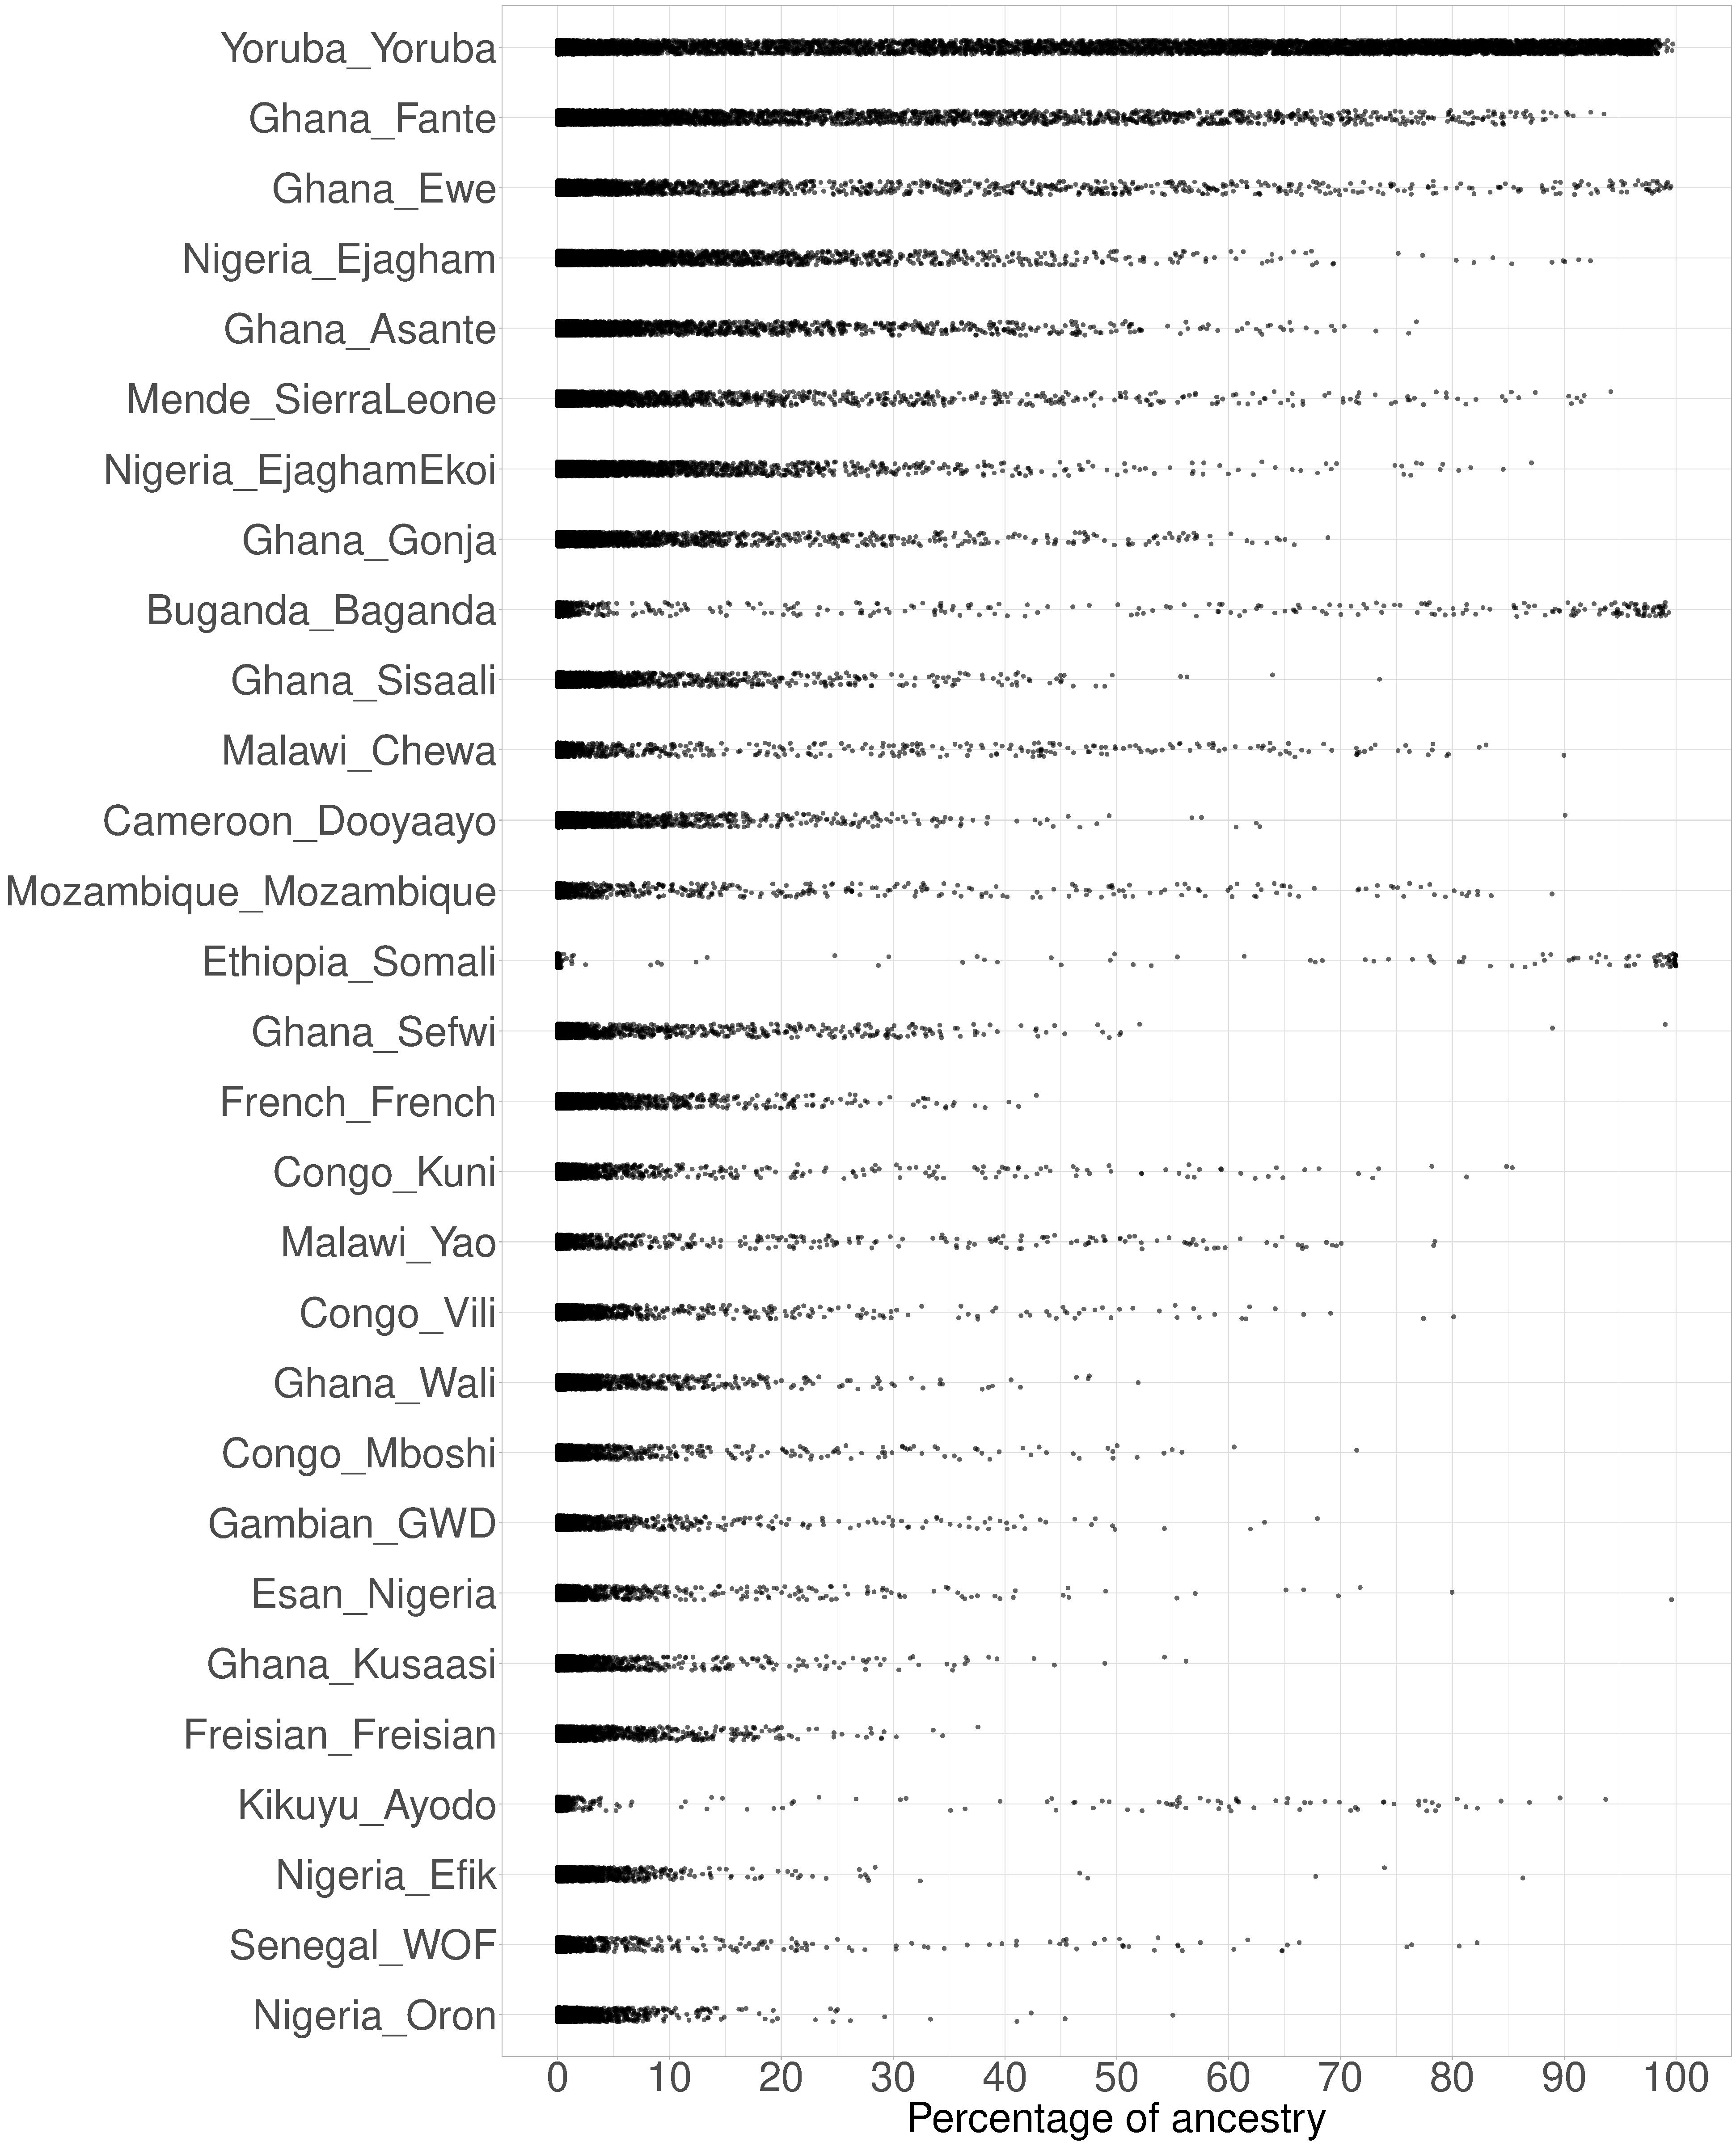
\includegraphics[width=1.0\textwidth]{../images/chapter3/SF_props_distribution_top30.pdf}
%    \caption{The 30 Human Origins populations which have the highest contribution to all U.K. Biobank individuals with at least 50\% African Ancestry, based on SOURCEFIND analysis. Each row of points contains 8476 individuals and their position corresponds to the percentage of ancestry from that population. }
%    \label{fig:SF_props_distribution_top30}
%\end{figure}

\subsection{Verifying painting accuracy}

Not all individuals within the U.K. Biobank were born in the U.K.; visualising the ancestry distribution of these individuals may reveal insights into population history. I subsetted the coancestry matrix to contain only individuals who have data on birth location (6153/8472). We would expect that individuals who were born in a particular country would copy the most from reference populations from that country. For example, we would expect individuals who were born in South Africa to copy the most from sampled Bantu and Zulu ethnic groups from South Africa. This may not always be the case, as some ethnic groups have crossed borders in their history, but it should broadly be true.

\begin{figure}[htp]
    \centering
    \includegraphics[width=1.0\textwidth]{../images/chapter3/haplotype_map_SouthAfrica.pdf}
    \caption{Map of haplotype donation to U.K. Biobank individuals born in South Africa. Each point represents one Human Origins population, coloured according to the summed amount of chunklengths that population donates to all U.K. Biobank individuals born in South Africa. }
    \label{fig:haplotype_map_SouthAfrica}
\end{figure}

Fig. \ref{fig:haplotype_map_SouthAfrica} shows the map of haplotype donation from reference groups to U.K. Biobank individuals born in South Africa. It is clear that reference populations from South Africa, in particular the Zulu ethnic group, contribute the most to these individuals. The pattern is qualitatively the same for all countries which had a reasonable number of donor populations, suggesting that the painting had good resolution down to at least the level of individual countries.

There are several interesting results. For example, there are 2,263 individuals who were born in the Caribbean. Visualising the haplotype donation map for these individuals shows that they are primarily of West African ancestry {\color{red}[FIGURE??]}, consistent with historical evidence \cite{micheletti2020genetic}. Individuals born in Brazil have ancestry from further South, again consistent with historical evidence (citation needed). However, it should be noted that there is a relatively small sample size from individuals born in Brazil (n=9), and that these individuals may not be representative of the Brazilian population. 

As a formal test of the painting accuracy, I estimated SOURCEFIND ancestry proportions in each retained U.K. Biobank individual. An individual was `assigned' to a particular ethnic group if they had {\color{red}75\%[NOT CLEAR THIS IS BEST -- WORTH HAVING A PLOT OF PREDICTION ACCURACY VS \% THRESHOLD?]} or more ancestry from that group. If the country the assigned reference population is from matches the birth location of the individual, then I considered that a `success' and a `fail' otherwise. Individuals who were born in the U.K. or who had no birth country were excluded from this analysis. 

\begin{figure}[htp]
    \centering
    \includegraphics[width=1.0\textwidth]{../images/chapter3/country_of_origin_allInds.pdf}
    \caption{Correspondence of true birth country with estimated birth country. Each bar corresponds to a true birth country, with the length of the bar corresponding to the total number of people in our dataset born in that country. The green section corresponds to the total number of individuals where the birth country was correctly guessed and the red section to those who were incorrectly guessed. Percentage labels give percentage correct for that country.}
    \label{fig:country_of_origin_allInds}
\end{figure}

The overall accuracy at predicting birth location was 81.63\%, suggesting there was substantial information within the coancestry matrix. For the countries where there was {\color{red}a large number of reference populations[NOT CLEAR THIS IS RELATED -- GIVEN YOU SHOWED THAT NIGERIA MATCHES PRIMARILY TO ONLY ONE GROUP]}, such as Ghana and Nigeria, the prediction accuracy was high. For certain countries, the prediction accuracy was much lower. For example, Tanzania, which is only represented by a single reference population, had a prediction match of XX\%. Zimbabwe had by far the lowest prediction accuracy (14\%) out of countries with more than {\color{red}100 individuals[DO YOU MEAN REF INDIVIDUALS OR UK BIOBANK INDIVIDUALS?]}. Of the 266 individuals born in Zimbabwe, 194 were assigned to an ethnic group from outside Zimbabwe; 74 to Malawi\_Chewa, 71 to Mozambique\_Mozambique and 49 to Malawi\_Yao. Individuals from the ethnic groups from Malawi are found across Malawi, Zimbabwe and other countries, showing the possible weakness of this approach which aims to categorise individuals into a single country, as ethnic groups often transcend countries. 

I also performed the same analysis but using the data which had been imputed. This stands as a practical test of whether it is preferable to impute or retain a smaller number of non-imputed SNPs. This yielded an accuracy of 81.89\%, a value almost identical to that obtained with the dataset containing approximately 70,000 non-imputed SNPs.{\color{red}[I THINK YOU WANT MORE HERE, AS THIS CONTRADICTS THE POINT YOU ARE TRYING TO MAKE ABOUT IMPUTATION BEING BAD. FOR EXAMPLE, ``Despite my earlier results indicating that SOURCEFIND results are less accurate if using imputed data due to reference bias...'' WOULD ALSO BE GOOD TO KNOW WHERE THEY DIFFER; FOR WHICH POPS IF AT ALL (E.G. MAYBE A SCATTERPLOT OF ACCURACIES UNDER THE TWO CASES)]}


\subsection{Patterns of African ancestry across the U.K.}

The U.K. Biobank dataset also contains data on the testing centre that each individual registered at. I used this information to see whether there was structure in how different ethnicities are distributed across the U.K. There was no apparent outliers in terms of centers and the proportion of individuals who had at least 50\% African ancestry (Fig. \ref{fig:country_of_origin_allInds}). No clear pattern was apparent, other than Yoruba ancestry dominating most centres. 
 
I also estimated the information entropy{\color{red}[HOW DID YOU CALCULATE THIS? DOES THIS INCLUDE EUROPEAN ANCESTRY?]} of each centre based on the SOURCEFIND proportions, {\color{red}analogous to previous work done on European ancestry in UK Biobank individuals (S.Hu, personal communication)}. In this context, information entropy can be seen as analagous to the amount of diversity in different ancestries present in a particular centre. The two centres in the two largest metropolitan areas, London and Birmingham, have the largest amount of entropy{\color{red}[HOW MUCH SO? SHOULD HIGHLIGHT LONDON ON THE FIG -- IS CROYDON A MISTAKE?]}, suggesting that ethnic diversity is greater in larger cities.

\begin{sidewaysfigure}[htp]
    \centering
    \includegraphics[width=1.0\textwidth]{../images/chapter3/SF_props_pie_chart.pdf}
    \caption{Distribution of ethnicities across different testing centres. Each pie corresponds to a U.K. Biobank testing centre, with each section of the each pie corresponding to a different ethnicity.}
    \label{fig:country_of_origin_allInds}
\end{sidewaysfigure}

